\documentclass[tikz,14pt,fleqn]{article}


\usepackage[utf8]{inputenc}
\usepackage[margin=1in]{geometry}
\usepackage[titletoc,title]{appendix}
\usepackage{latexsym}
\usepackage{amssymb}
\usepackage{gensymb}
\usepackage{amsmath}
\usepackage{amsfonts}
\usepackage[dvipsnames]{xcolor}
\usepackage{multicol}
\usepackage{graphicx}
\usepackage{fancyhdr}
\usepackage[linguistics]{forest}
\usepackage{colortbl}
\usepackage{pdfpages}
\usepackage{wrapfig}
\usepackage{cleveref}
\usepackage{cancel}

% to fixme
\usepackage{xcolor} 
\definecolor{FIXMECOLOR}{rgb}{1,0,0}
\newcommand{\FIXME}[1]{{\color{FIXMECOLOR}{\textbf{FIXME: #1}}}} 

% to simplify math 
\newcommand{\pvec}[3]{
   \ensuremath{
   \begin{pmatrix}
       #1 \\
       #2 \\
       #3
   \end{pmatrix}
}}

\newcommand{\bvec}[3]{
   \ensuremath{
   \begin{bmatrix}
       #1 \\
       #2 \\
       #3
   \end{bmatrix}
}}

\newcommand{\bmat}[1]{
   \ensuremath{
   \begin{bmatrix}
       #1
   \end{bmatrix}
}}

\newcommand{\dotprod}[2]{\ensuremath{\left< #1, #2 \right>}}

%% For plotting
\usepackage{pgfplots}
\pgfplotsset{width=10cm,compat=1.9}
\usepgfplotslibrary{external}
\tikzexternalize
%%
\usepackage{dirtree}
\usepackage{subcaption}
\usepackage{xifthen}% provides \isempty test
\usepackage{glossaries}

\captionsetup[subfigure]{labelformat=empty}
\definecolor{color1}{HTML}{0B0C10}
\definecolor{color2}{HTML}{1F2833}
\definecolor{color3}{HTML}{C5C6C7}
\definecolor{color4}{HTML}{66FCF1}
\definecolor{color5}{HTML}{45A29E}

\pagestyle{fancy}
\fancyhf{}
%%%%%%%%%%%%%%%%%%%%%%%%%%%%
%% VARIABLES
\newcommand\namesurname{Albert Cerfeda\\Alessandro Gobbetti}
\newcommand\assignment{Assignment 4}

\newcommand\subject{Computer Graphics}
\newcommand\documentdate{18.10.2022}

% Title content
%%%%%%%%%%%%%%%%%%%%%%%%%%%%
\rhead{\assignment}
\lhead{\namesurname}
%%%%%%%%%%%%%%%%%%%%%%%%%%%%
\rfoot{Page \thepage}
\setlength{\parindent}{0pt}

\newcommand\xdownarrow[1][2ex]{%
   \mathrel{\rotatebox{90}{$\xleftarrow{\rule{#1}{0pt}}$}}
}

\begin{document}

\begin{titlepage}
   \begin{center}
       \vspace*{1cm}

       \textbf{\Large{Homework Assignment}}

       \vspace{0.5cm}
        \textbf{\subject}\\[5mm]
       \assignment
        
            
       \vspace{1.8cm}

        \namesurname
       \tableofcontents

       \vspace*{\fill}
     
        
\includegraphics[width=0.4\textwidth]{fig/logo.png}
       
        \documentdate \\
        Università della Svizzera italiana\\
        Faculty of Informatics\\
        Switzerland\\

   \end{center}
\end{titlepage}



\section{Exercise 1}
\subsection{Task 1}
\[
R_{90} = 
\begin{bmatrix}
cos(\alpha) & -sin(\alpha) & 0\\
sin(\alpha) & cos(\alpha) & 0\\
0 & 0 & 1
\end{bmatrix} = 
\begin{bmatrix}
cos(90) & -sin(90) & 0\\
sin(90) & cos(90) & 0\\
0 & 0 & 1
\end{bmatrix} =
\begin{bmatrix}
0 & -1 & 0\\
1 & 0 & 0\\
0 & 0 & 1
\end{bmatrix}
\]

% translation matrix T
\[
T =
\begin{bmatrix}
1 & 0 & 1\\
0 & 1 & -2\\
0 & 0 & 1
\end{bmatrix}
\]


\subsection{Task 2}
Represent $p_1 = (1, 1)^T$ and $p = (1.5, 2.5)^T$ and $u = p - p_1 = (0.5, 1.5)^T$ in homogeneous coordinates:
\[
p_1 = (1,1,1)^T, \quad p = (1.5,2.5,1)^T, \quad u = (0.5,1.5,0)^T
\]
Rotate the points and the vector:
\[
R_{90} \cdot p_1=
\begin{bmatrix}
0 & -1 & 0\\
1 & 0 & 0\\
0 & 0 & 1
\end{bmatrix}
\begin{bmatrix}
1\\
1\\
1
\end{bmatrix}=
\begin{bmatrix}
-1\\
1\\
1
\end{bmatrix}
\quad p_{1_{90}} = (-1,1)^T
\]

\[
R_{90} \cdot p=
\begin{bmatrix}
0 & -1 & 0\\
1 & 0 & 0\\
0 & 0 & 1
\end{bmatrix}
\begin{bmatrix}
1.5\\
2.5\\
1
\end{bmatrix}=
\begin{bmatrix}
-2.5\\
1.5\\
1
\end{bmatrix}
\quad p_{90} = (-2.5, 1.5)^T
\]

\[
R_{90} \cdot u=
\begin{bmatrix}
0 & -1 & 0\\
1 & 0 & 0\\
0 & 0 & 1
\end{bmatrix}
\begin{bmatrix}
0.5\\
1.5\\
0
\end{bmatrix}=
\begin{bmatrix}
-1.5\\
0.5\\
0
\end{bmatrix}
\quad u_{90} = (-1.5, 0.5)^T
\]

Translate the rotated points and vector:
\[
T \cdot p_{1_{90}}=
\begin{bmatrix}
1 & 0 & 1\\
0 & 1 & -2\\
0 & 0 & 1
\end{bmatrix}
\begin{bmatrix}
-1\\
1\\
1
\end{bmatrix}=
\begin{bmatrix}
0\\
-1\\
1
\end{bmatrix}
\quad p'_1 = (0,-1)^T
\]

\[
T \cdot p_{90}=
\begin{bmatrix}
1 & 0 & 1\\
0 & 1 & -2\\
0 & 0 & 1
\end{bmatrix}
\begin{bmatrix}
-2.5\\
1.5\\
1
\end{bmatrix}=
\begin{bmatrix}
-1.5\\
-0.5\\
1
\end{bmatrix}
\quad p' = (-1.5,-0.5)^T
\]

\[
T \cdot u_{90}=
\begin{bmatrix}
1 & 0 & 1\\
0 & 1 & -2\\
0 & 0 & 1
\end{bmatrix}
\begin{bmatrix}
-1.5\\
0.5\\
0
\end{bmatrix}=
\begin{bmatrix}
-1.5\\
0.5\\
0
\end{bmatrix}
\quad u' = (-1.5,0.5)^T
\]

Verify that $u' = p' - p'$:
\[
   p' - p'_1
   =
   \begin{bmatrix}
   -1.5\\
   -0.5\\
   \end{bmatrix}
   -
   \begin{bmatrix}
   0\\
   -1\\
   \end{bmatrix}
   =
   \begin{bmatrix}
   -1.5\\
   0.5\\
   \end{bmatrix}
   =
   u'
\]

Since $u$ is a vector, it is not affected by the translation. Thus, $u' = u$.

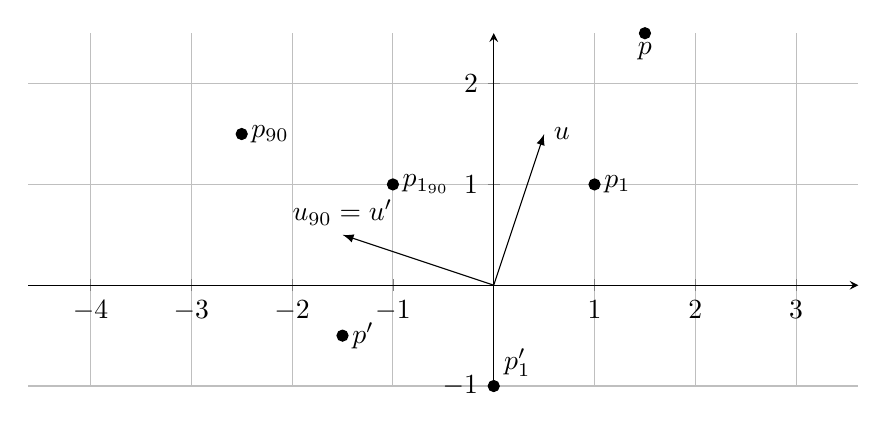
\begin{tikzpicture}
   \begin{axis}[axis lines=middle,axis equal,grid=both,width=\textwidth, height=0.5\textwidth]
      \addplot[mark=*,only marks] coordinates {(1,1)} node[right] {$p_1$};
      \addplot[mark=*,only marks] coordinates {(1.5,2.5)} node[below] {$p$};
      \addplot[mark=,->,>=latex] coordinates {(0,0) (0.5,1.5)} node[right] {$u$};
      
      \addplot[mark=*,only marks] coordinates {(-1,1)} node[right] {$p_{1_{90}}$};
      \addplot[mark=*,only marks] coordinates {(-2.5,1.5)} node[right] {$p_{90}$};
      
      \addplot[mark=*,only marks] coordinates {(0,-1)} node[above, xshift=0.3cm] {$p'_1$};
      \addplot[mark=*,only marks] coordinates {(-1.5,-0.5)} node[right] {$p'$};
      
      \addplot[mark=,->,>=latex] coordinates {(0,0) (-1.5,0.5)} node[above] {$u_{90} = u'$};
   \end{axis}
\end{tikzpicture}


\subsection{Task 3}

Scaling matrix:
\[
S = \begin{bmatrix}
2 & 0 & 0\\
0 & 2 & 0\\
0 & 0 & 1
\end{bmatrix}
\]

\[
S \cdot p'_1= 
\begin{bmatrix}
2 & 0 & 0\\
0 & 2 & 0\\
0 & 0 & 1
\end{bmatrix}
\begin{bmatrix}
0\\
-1\\
1
\end{bmatrix}=
\begin{bmatrix}
0\\
-2\\
1
\end{bmatrix}
\quad p''_1 = (0,-2)^T
\]

\[
S \cdot p'=
\begin{bmatrix}
2 & 0 & 0\\
0 & 2 & 0\\
0 & 0 & 1
\end{bmatrix}
\begin{bmatrix}
-1.5\\
-0.5\\
1
\end{bmatrix}=
\begin{bmatrix}
-3\\
-1\\
1
\end{bmatrix}
\quad p'' = (-3,-1)^T
\]

\[
S \cdot u'=
\begin{bmatrix}
2 & 0 & 0\\
0 & 2 & 0\\
0 & 0 & 1
\end{bmatrix}
\begin{bmatrix}
-1.5\\
0.5\\
0
\end{bmatrix}=
\begin{bmatrix}
-3\\
1\\
0
\end{bmatrix}
\quad u'' = (-3,1)^T
\]

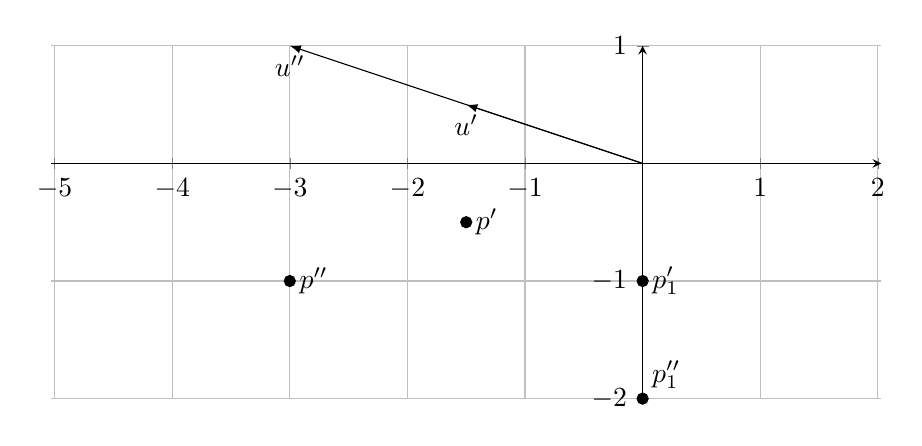
\begin{tikzpicture}
    \begin{axis}[axis lines=middle,axis equal,grid=both,width=\textwidth, height=0.5\textwidth]
        \addplot[mark=*,only marks] coordinates {(0,-1)} node[right] {$p'_1$};
        \addplot[mark=*,only marks] coordinates {(-1.5,-0.5)} node[right] {$p'$};
        \addplot[mark=,->,>=latex] coordinates {(0,0) (-1.5,0.5)} node[below] {$u'$};
        
        \addplot[mark=*,only marks] coordinates {(0,-2)} node[above, xshift=0.3cm] {$p''_1$};
        \addplot[mark=*,only marks] coordinates {(-3,-1)} node[right] {$p''$};
        \addplot[mark=,->,>=latex] coordinates {(0,0) (-3,1)} node[below] {$u''$};
   \end{axis}
\end{tikzpicture}



\subsection{Task 4}

Compute inverse matrix of $S$:
\[
S^{-1} = \begin{bmatrix}
\frac{1}{2} & 0 & 0\\
0 & \frac{1}{2} & 0\\
0 & 0 & 1
\end{bmatrix}
\]
Compute inverse matrix of $T$:
\[
T^{-1} = \bmat{
1 & 0 & -1\\ 
0 & 1 & 2\\
0 & 0 & 1
}
\]
Compute inverse matrix of $R_{90}$:
\[
R_{90}^{-1} = \bmat{
0 & 1 & 0\\ 
-1 & 0 & 0\\
0 & 0 & 1
}
\]
Compute inverse transformation matrix $M$:
\begin{align*}
M &= R_{90}^{-1} T^{-1} S^{-1} \\
&=\bmat{
0 & 1 & 0\\ 
-1 & 0 & 0\\
0 & 0 & 1
}\cdot\bmat{
1&0&-1\\
0&1&2\\
0&0&1
}\cdot\bmat{
\frac{1}{2}&0&0\\
0&\frac{1}{2}&0\\
0&0&1} \\
&= \bmat{0&1&2\\ -1&0&1\\ 0&0&1}\cdot \bmat{\frac{1}{2}&0&0\\ 0&\frac{1}{2}&0\\ 0&0&1}\\
&= \bmat{0&\frac{1}{2}&2\\ -\frac{1}{2}&0&1\\ 0&0&1}
\end{align*}

\newcommand{\M}[0]{
\bmat{0&\frac{1}{2}&2\\ -\frac{1}{2}&0&1\\ 0&0&1}
}


\begin{align*}
p_1 &= M p_{1}^{''}\\
&= \M \cdot \bmat{0\\-2\\1} = \bmat{1\\ 1\\ 1}\rightarrow \bmat{1\\1}\checkmark
\end{align*} 
\begin{align*}
p &= M p^{''}\\
&= \M \cdot \bmat{-3\\-2\\1} = \bmat{1.5\\2.5\\1}\rightarrow \bmat{1.5\\2.5}\checkmark
\end{align*} 
\begin{align*}
u &= M u^{''}\\
&= \M \cdot \bmat{-3\\1\\0}\\
&= \bmat{0.5\\1.5\\0} \rightarrow \bmat{0.5\\1.5}\checkmark
\end{align*} 


\section{Exercise 2}

% Consider a triangle made of three points p1 = (6, 0, 4), p2 = (2, 0, 0), and p3 = (2, 4, 4). 
% Verify whether point p = (4, 1, 3) belongs to the interior of the triangle

\[
   p_1 = (6, 0, 4),\quad p_2 = (2, 0, 0),\quad p_3 = (2, 4, 4)
\]
\[
   p = (4, 1, 3)
\]

Signed area of triangle [$p_1$, $p_2$, $p_3$]:
\[
   n = (p_2 - p_1) \times (p_3 - p_1) = 
   \left(
   \pvec{2}{0}{0} - \pvec{6}{0}{4}
   \right)
   \times
   \left(
   \pvec{2}{4}{4} - \pvec{6}{0}{4}
   \right) =
   \pvec{-4}{0}{-4}
   \times
   \pvec{-4}{4}{0}
   =
   \pvec{16}{16}{-16}
\]


Normals of the sub-triangles:
\[
   n_1 = (p_3 - p) \times (p_1 - p) =
   \left(
   \pvec{2}{4}{4} - \pvec{4}{1}{3}
   \right)
   \times
   \left(
   \pvec{6}{0}{4} - \pvec{4}{1}{3}
   \right) =
   \pvec{-2}{3}{1}
   \times
   \pvec{2}{-1}{1}
   =
   \pvec{4}{4}{-4}
\]



\[
   n_2 = (p_1 - p) \times (p_2 - p) =
   \left(
   \pvec{6}{0}{4} - \pvec{4}{1}{3}
   \right)
   \times
   \left(
   \pvec{2}{0}{0} - \pvec{4}{1}{3}
   \right) =
   \pvec{2}{-1}{1}
   \times
   \pvec{-2}{-1}{-3}
   =
   \pvec{4}{4}{-4}
\]


\[
  n_3 = (p_2 - p) \times (p_3 - p) =
   \left(
   \pvec{2}{0}{0} - \pvec{4}{1}{3}
   \right)
   \times 
   \left(
   \pvec{2}{4}{4} - \pvec{4}{1}{3}
   \right) =
   \pvec{-2}{-1}{-3}
   \times
   \pvec{-2}{3}{1}
   =
   \pvec{8}{8}{-8}
\]


Then compute the signs between the obtained sub-triangles normals with the normal of the triangle:
\[
   sign(\dotprod{n_1}{n}) = 
   sign
   \left(
   \dotprod{\pvec{4}{4}{-4}}{\pvec{16}{16}{-16}}
   \right) = 
   sign(64 + 64 + 64 ) = sign(192) = +1
\]

\[
   sign(\dotprod{n_2}{n}) = 
   sign
   \left(
   \dotprod{\pvec{4}{4}{-4}}{\pvec{16}{16}{-16}}
   \right) = 
   sign(64 +64 +64 ) = sign(192) = +1
\]

\[
   sign(\dotprod{n_3}{n}) = 
   sign
   \left(
   \dotprod{\pvec{8}{8}{-8}}{\pvec{16}{16}{-16}}
   \right) = 
   sign(128 + 128 + 128) = sign(384) = +1
\]

Since every sign is positive, the point is inside the triangle.

\newpage

\section{Exercise 3}
The centroid of the triangle is the point where the medians meet.
The medians are the lines that connect the vertices of the triangle to the midpoint of the opposite side.

Consider points $A$, $B$, $C$ as vertices of a triangle and as barycentric coordinate system for the plane.
Then every point on the plain can be expressed as $\left( \alpha, \beta, \gamma \right)$ with $\alpha+\beta+\gamma=1$.

Now, consider the three medians of the triangle, $AM_A$, $BM_B$, $CM_C$, connecting the vertices to the midpoint $M_A$, $M_B$, and $M_C$.

$M_A$ is defined in barycentric coordinates as $\left( \alpha, \beta, \gamma \right)$ where $\beta = \gamma$.
Following the same reasoning, $M_B$ is defined as $\left( \alpha, \beta, \gamma \right)$ where $\alpha = \gamma$ and $M_C$ as $\left( \alpha, \beta, \gamma \right)$ where $\alpha = \beta$.

Thus, to find the centroid of a triangle we have to find the point where the medians meet:
\begin{equation}
   \begin{cases}
      \alpha + \beta + \gamma = 1 \\
      \beta = \gamma \\
      \alpha = \gamma \\
      \alpha = \beta
   \end{cases}
   \Rightarrow
   \begin{cases}
      \alpha + \beta + \gamma = 1 \\
      \alpha = \beta = \gamma \\
   \end{cases}
   \Rightarrow
   \alpha = \beta = \gamma = \frac{1}{3}
\end{equation}

So we can represent the centroid of a triangle as $\left({\frac{1}{3}}, {\frac{1}{3}}, {\frac{1}{3}} \right)$.


Since barycentric coordinates of points inside the triangle are between $0$ and $1$ 
we can conclude that the centroid of the triangle divides the medians in $\frac{2}{3}:\frac{1}{3}$ ratio, better written as $2:1$ ratio.







\section{Exercise 4}
We know that given a homogeneous coordinate $h = \bmat{a\\b\\c}$, the cartesian coordinate counterpart $f$ is obtained by dividing every element by the extra dimension value and discarding such dimension $f = \bmat{\frac{a}{c}\\\frac{b}{c}}$\\
By looking at the graph we can deduce that given any point $p$, its transformed counterpart equals $p'' = \bmat{1\\\frac{y}{x}}$.\\
Let us write the point transformation as a matrix multiplication:
\[
p''  = \bmat{a&b&c\\d&e&f\\g&h&i} \cdot \bmat{p_x\\p_y\\p_z} = \bmat{1\\\frac{p_y}{p_x}\\1}
\]
We can intuitively deduce that in order for $p''_x$ to equal $1$ we have to divide and therefore simplify $p_x$ by $p_x$ itself. Since we know that in order to convert homogeneous coordinates to cartesian we have to divide all the elements by the third element, we can conveniently set $p_z$ to equal $p_x$ in order to make the before-mentioned simplification take place.
\[
p''  = \bmat{1&b&c\\d&e&f\\1&h&i} \cdot \bmat{p_x\\p_y\\p_x} = \bmat{\frac{p_x}{p_x}\\\frac{1}{p_x}\\\frac{p_x}{p_x}} = \bmat{1\\\frac{1}{p_x}\\1}
\]
Finally we set $e = 1$ in order to preserve the value of $y$, like so:
\[
p''  = \bmat{1&b&c\\d&1&f\\1&h&i} \cdot \bmat{p_x\\p_y\\p_x} = \bmat{1\\\frac{p_y}{p_x}\\1}
\]
The transformation matrix is $S = \bmat{1&0&0\\0&1&0\\1&0&0}\forall p_x \in \mathds{R}, p_x \neq 0$\\
In the case where point $p$ lies on the y-axis (ie $p_x = 0$) there isn't a valid solution, as $p''_y$ would involve a division by $0$.

\section{Bonus exercise 5}

\begin{equation}
   \begin{cases}
      y = ax + b \\
      y = \frac{p_y}{p_x} x
   \end{cases}
   \Rightarrow
   \begin{cases}
      x = \frac{bp_x}{p_y - ap_x} \\
      y = \frac{bp_y}{p_y - ap_x}
   \end{cases}
\end{equation}
From this we know that:
\[
   \frac{m_{11}x + m_{12}y + m_{13}}{m_{31}x + m_{32}y + m_{33}} = \frac{bp_x}{p_y - ap_x}
\]
and
\[
   \frac{m_{21}x + m_{22}y + m_{23}}{m_{31}x + m_{32}y + m_{33}} = \frac{bp_y}{p_y - ap_x}
\]

Thus we obtained that: 
\[
   \begin{bmatrix}
      m_{11} & m_{12} & m_{13} \\
      m_{21} & m_{22} & m_{23} \\
      m_{31} & m_{32} & m_{33}
   \end{bmatrix}
   = 
   \begin{bmatrix}
      b & 0 & 0 \\
      0 & b & 0 \\
      -a & 1 & 0
   \end{bmatrix}
\]


\end{document}